\section{Tasso di Trasmissione e Criteri di Decodifica}
Come anticipato, la codifica di canale affronta il problema dell'inaffidabilità introducendo ridondanza controllata, allo scopo di proteggere l'informazione dal rumore e abbattere la probabilità di errore a destinazione.

\subsection{Codici di Canale e Tasso di Trasmissione}
Per quantificare l'efficienza di questa operazione, definiamo alcune metriche fondamentali.
Sia $C$ un codice su un alfabeto $q$-ario:
\begin{itemize}
    \item $n$ è la lunghezza delle parole di codice (codeword) emesse sul canale.
    \item $M = |C|$ è la cardinalità del codice, ovvero il numero di codeword valide.
\end{itemize}

Poiché il numero totale di sequenze possibili di lunghezza $n$ è $q^n$, per poter identificare e correggere gli errori è necessario scegliere un sottoinsieme ristretto di codeword valide, imponendo $M < q^n$ (e quindi $\log_q M < n$). Questo evita che il rumore trasformi inevitabilmente una codeword in un'altra codeword legittima.

Si definisce il \textbf{tasso di trasmissione del codice} (o \textit{code rate}) $R$ come:
\[ R = \frac{\log_q M}{n} = \frac{k}{n} \quad \left[\frac{\text{simboli di sorgente}}{\text{simboli di canale}}\right] \]
dove $k = \log_q M$ rappresenta il numero equivalente di simboli di informazione pura trasportati da ciascuna codeword. A causa dell'aggiunta di ridondanza ($k < n$), il tasso risulta sempre $R < 1$.

\paragraph{L'approccio della ridondanza: esempio della decodifica a maggioranza}
Per dimostrare matematicamente come l'aggiunta di ridondanza abbatta la probabilità di errore, consideriamo la trasmissione su un Canale Binario Simmetrico (BSC) con probabilità di errore sul singolo bit pari a $\epsilon$. Senza alcuna codifica, la probabilità di ricevere un simbolo errato è banalmente $P_e = \epsilon$.

Introduciamo un semplice \textbf{codice a ripetizione} con $n=3$: il simbolo di sorgente $0$ viene codificato e trasmesso come $000$, mentre il simbolo $1$ come $111$. Il tasso del codice scende drasticamente a $R = 1/3$.

In ricezione, applichiamo un criterio di \textbf{decodifica a maggioranza}: il blocco di 3 bit ricevuto viene decodificato nel simbolo che compare più volte. Di conseguenza, si verificherà un errore di decodifica solo se il canale altera 2 o 3 bit della codeword.
Essendo il canale senza memoria, gli errori sui bit sono eventi statisticamente indipendenti. La probabilità di errore dell'intero blocco è data dalla somma dei termini della distribuzione binomiale:
\[ P_e = \binom{3}{2}\epsilon^2(1-\epsilon) + \binom{3}{3}\epsilon^3 = 3\epsilon^2(1-\epsilon) + \epsilon^3 \]
Ipotizzando un canale con $\epsilon = 10^{-2}$, la probabilità di errore post-decodifica scende a $P_e \approx 3 \cdot 10^{-4}$. L'inserimento della ridondanza ha sacrificato la velocità di trasmissione per ottenere un drastico guadagno sull'affidabilità.



\subsection{Il Decodificatore di Canale}
Poiché, grazie alla ridondanza, lo spazio delle possibili sequenze in uscita $Y$ è molto più ampio dell'insieme delle $M$ parole di codice in ingresso $X$, il ricevitore non può operare una semplice corrispondenza biunivoca. Il decodificatore \textit{raggruppa} le sequenze ricevute in $M$ \textbf{classi di equivalenza} dello spazio $Y$.
\\
Formalmente, si definiscono:
\begin{itemize}
    \item \textbf{Funzione di decodifica} $\Psi: Y \rightarrow X$: associa ad ogni parola in uscita $y$, un elemento stimato $\tilde{x} \in X$.
    \item $M$ \textbf{Regioni di decodifica}: $R_i$ è la regione composta da tutti gli $y$ tali che $\Psi(y) = x_i$.
\end{itemize}
\noindent
Le $M$ regioni $R_1, \dots, R_M$ costituiscono classi di equivalenza che partizionano l'intero spazio di arrivo $Y$.

\begin{minipage}{0.45\textwidth}
    \raggedright \large
    Introduce una \textbf{partizione} in $M$ classi di equivalenza $\mathcal{R}_1, \dots, \mathcal{R}_M$ su $Y$.
\end{minipage}
\hfill
\begin{minipage}{0.5\textwidth}
    \centering
    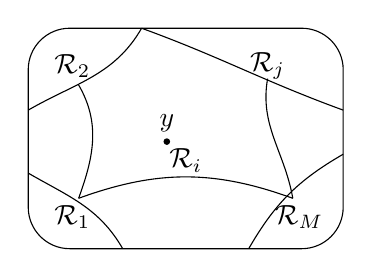
\begin{tikzpicture}[scale=0.8]
        \draw[rounded corners=15pt] (0,0) rectangle (5,3.5);

        \draw (0, 2.2) to[out=30, in=240] (1.8, 3.5);
        \draw (0, 1.2) to[out=-30, in=120] (1.5, 0);
        \draw (3.5, 0) to[out=60, in=210] (5, 1.5);
        \draw (1.8, 3.5) to[out=-20, in=160] (5, 2.2);

        % Linee interne per definire Ri
        \draw (0.8, 2.6) to[out=300, in=70] (0.8, 0.8);
        \draw (0.8, 0.8) to[out=20, in=160] (4.2, 0.8);
        \draw (4.2, 0.8) to[out=100, in=260] (3.8, 2.7);

        % Etichette delle regioni
        \node at (0.7, 2.9) {$\mathcal{R}_2$};
        \node at (0.7, 0.5) {$\mathcal{R}_1$};
        \node at (4.3, 0.5) {$\mathcal{R}_M$};
        \node at (3.8, 2.9) {$\mathcal{R}_j$};
        \node at (2.5, 1.4) {$\mathcal{R}_i$};

        \fill (2.2, 1.7) circle (1.5pt) node[above] {$\bm{y}$};

    \end{tikzpicture}
\end{minipage}

Con questa impostazione, un \textbf{errore di decodifica} si verifica quando viene trasmesso il simbolo $x_i \in X$, ma a causa del rumore si riceve una sequenza $y$ che cade al di fuori della sua regione di competenza (cioè $y \notin R_i$). 
Per una data parola $x_i$, la probabilità che ciò avvenga è:
\[P_{err}= \sum_{i=1}^M p(x_i)P_{err}(x_i)=\sum_{i=1}^M p(x_i) \sum_{y \notin R_i}p(y|x_i)\]


Analizzando la formulazione finale, emergono considerazioni fondamentali per il progetto del sistema di codifica di canale:
\begin{itemize}
    \item $p(x_i)$ dipende dalla sorgente
    \item $p(y|x_i)$ dipende dal canale
\end{itemize}
L'unico fattore su cui incide la codifica/decodifica è $R_i$. L'obiettivo sarà quindi scegliere le \textbf{regioni di decodifica $R_1, \dots, R_M$} per minimizzare $P_{err}$





\subsection{Criteri di Decisione Ottimi}
Come discusso in precedenza, l'obiettivo primario di un decodificatore è definire le regioni $R_i$ in modo da rendere minima la probabilità di errata decodifica globale. I \textbf{criteri di decisione ottimi} forniscono proprio le regole matematiche per tracciare i confini di queste regioni nel modo più efficiente possibile, a seconda delle informazioni disponibili sul sistema.

\subsubsection{Criterio dell'Osservatore Ideale}
Il Criterio dell'Osservatore Ideale è la regola di decisione ottima in senso assoluto. 
L'obiettivo è \textbf{minimizzare la probabilità di errore media} del sistema, massimizzando di conseguenza la probabilità di \textbf{corretta decodifica a posteriori}.

Ad ogni sequenza ricevuta $y$ è associata la probabilità di commettere un errore scegliendo una generica parola stimata $\tilde{x}$. Questa probabilità a posteriori è:
\[ P_e(y) = Pr(\tilde{x} \neq x | y) = 1 - Pr(\tilde{x} = x | y) \]

Mediando su tutte le possibili sequenze in uscita, la probabilità di errore totale del sistema diventa:
\[ P_e = \sum_j p(y_j) P_e(y_j) = 1 - \sum_j p(y_j) Pr(\tilde{x} = x | y_j) \]

La probabilità $p(y_j)$ di ricevere una determinata sequenza dipende unicamente dalla combinazione tra sorgente e canale ($p(y_j) = \sum_i p(x_i)p(y_j|x_i)$) e non dalla regola di decodifica. Pertanto, l'unico modo per \textbf{minimizzare} $P_e$ è \textbf{massimizzare} la probabilità di corretta decodifica a posteriori $Pr(\tilde{x} = x | y_j)$ per ogni singola osservazione $y_j$.

\paragraph{Regola di decisione}
Per ottenere questo obiettivo, il decodificatore seleziona la parola di codice $x_i$ che risulta essere la più probabile \textit{dopo} aver osservato l'uscita $y$. In formule, la parola stimata $\tilde{x}$ sarà:
\[ \tilde{x} = \operatorname*{argmax}_{x_i} p(x_i|y)\]
Questo significa che la funzione di decodifica assegnerà $y$ a $x_i$, ovvero $\Psi(y)=x_i$, se e solo se:
\[ p(x_i|y) \geq p(x_j|y) \quad \forall j \neq i \]

Applicando il Teorema di Bayes a questa disuguaglianza, otteniamo:
\[ \frac{p(y|x_i)p(x_i)}{p(y)} \geq \frac{p(y|x_j)p(x_j)}{p(y)} \]
Poiché il denominatore $p(y)$ è comune a entrambi i membri ed è sempre strettamente positivo, possiamo eliderlo senza alterare la disuguaglianza. La regola di decisione operativa diventa quindi: 
si ha $\Psi(y)=x_i$ se $\forall j \neq i$ risulta

\begin{center}
\begin{tikzpicture}[>=Stealth, node distance=0.6cm, baseline=(p1.base)]
    % --- 1. COSTRUZIONE EQUAZIONE (testo nero) ---
    % Scomponiamo l'equazione in pezzi per cerchiarli singolarmente
    \node (p1) {$p(x_i)$};
    \node (p2) [right=-2pt of p1] {$p(y|x_i)$};
    \node (rest) [right=0pt of p2] {$\geq p(x_j)p(y|x_j)$};

    % --- 2. CERCHIATURE ---
    % Sorgente (Azzurro)
    \node[draw=blue!50!black, fill=blue!10, ellipse, inner sep=1pt, 
          minimum width=1.2cm, minimum height=0.7cm, opacity=0.4] at (p1) {};
          
    % Canale (Giallino)
    \node[draw=orange!60!black, fill=yellow!20, ellipse, inner sep=1pt, 
          minimum width=1.6cm, minimum height=0.7cm, opacity=0.4] at (p2) {};

    % --- 3. DIDASCALIE E FRECCE ---
    % Nota SORGENTE a SINISTRA
    \node[left=1.2cm of p1, text=blue!80!black, font=\small, align=right] (txt_src) {dipende dalla\\sorgente};
    \draw[->, blue!80!black, thin] (txt_src.east) -- ([xshift=-8pt]p1.west);

    % Nota CANALE SOTTO
    \node[below=0.8cm of p2, text=orange!80!black, font=\small, align=center] (txt_chan) {dipende dal\\canale};
    \draw[->, orange!60!black, thin] (txt_chan.north) -- ([yshift=-8pt]p2.south);
    
\end{tikzpicture}
\end{center}


\vspace{0.2cm}
\noindent \colorbox{gray!15}{\textbf{Inconveniente:}} il decodificatore è progettato tenendo conto delle probabilità a priori $p(x_i)$, dipende quindi dalla specifica sorgente. In caso di modifica delle probabilità a priori il decodificatore deve essere \textit{tarato} nuovamente.

\subsubsection{Criterio di Massima Verosimiglianza (ML)}
Quando i messaggi in ingresso al canale sono equiprobabili (condizione che caratterizza un'uscita prodotta da una \textit{buona} codifica di sorgente a monte), si ottiene una semplificazione del Criterio dell'Osservatore Ideale. In questo caso, la distribuzione di probabilità a priori è \textbf{uniforme}:
\[ p(x_i) = \frac{1}{M} \quad \forall i \]

Applicando questa distribuzione di probabilità alla formula del Criterio dell'Osservatore Ideale ($p(y|x_i)p(x_i) \geq p(y|x_j)p(x_j)$) (sostituendo le probabilità a priori con $\frac{1}{M}$), il termine relativo alla sorgente è costante per ogni $i$ e si elide da entrambi i membri. La scelta ottima ricade quindi unicamente sul massimizzare la probabilità dipendente dal canale.

\paragraph{Regola di decisione}
Con questa premessa, il decodificatore, dalla sequenza ricevuta $y$, restituisce il messaggio $x_i$ se la probabilità che il canale abbia prodotto proprio $y$ a partire da $x_i$ (ovvero la sua \textbf{\textit{verosimiglianza}}) è maggiore rispetto a qualsiasi altro messaggio $x_j$.
\[ \Psi(y) = x_i \iff p(y|x_i) \geq p(y|x_j) \quad \forall j \neq i \]
La parola decodificata $\tilde{x} \in X$ sarà quindi tale che:
\[ \tilde{x} = \operatorname*{argmax}_{x_i} p(y|x_i)\]
Per progettare il decodificatore si lavora direttamente sulle colonne della matrice di transizione.

\noindent \colorbox{gray!15}{\textbf{Nota sull'ottimalità:}} La sua ottimalità assoluta è garantita \textit{solo} se i messaggi in ingresso sono perfettamente equiprobabili. Più la distribuzione effettiva si allontana dall'uniformità, più le prestazioni di questo criterio si allontanano dall'ottimo teorico.

\subsubsection{Criterio dell'Errore Massimale}
Questo criterio stabilisce a priori, per ogni codeword, un tetto massimo, $\delta$, alla probabilità di errata decodifica.
\[P_{err}\leq \delta \quad \forall i \in X\]
La probabilità media di errore sarà:

\[P_e=\sum_{i=1}^MP_{err}(x_i)p(x_i)\leq \delta\]
Non risulta però semplice implementare gli schemi di decodifica. Shannon ha usato questo criterio per \textit{spingere} il tasso di trasmissione al limite della capacità di canale.

\subsubsection{Esempi di criteri di decodifica}
% Esempio numerico dalle slide.
\paragraph{Esempio di osservatore ideale}
Si consideri lo schema di decisione dell'osservatore ideale applicato a un canale con 2 ingressi ($x_1, x_2$) e 3 uscite ($y_1, y_2, y_3$). Il canale è completamente definito dalla sua matrice di transizione $P$:
\begin{center}
    % --- Minipage Sinistra: Matrice di Transizione ---
    \begin{minipage}[c]{0.40\textwidth}
        \centering
        \renewcommand{\arraystretch}{2} % Spazio per le frazioni
        $P = \begin{bmatrix} 
            \frac{3}{4} & 0 & \frac{1}{4} \\ 
            0 & \frac{7}{8} & \frac{1}{8} 
        \end{bmatrix}$
    \end{minipage}
    \hfill
    % --- Minipage Destra: Diagramma del Canale ---
    \begin{minipage}[c]{0.50\textwidth}
        \centering
        \begin{tikzpicture}[yscale=1.2, xscale=1.5, >=Stealth]
            % Nodi di ingresso
            \node[left=5pt] (x1) at (0,0) {$x_1$}; \fill (0,0) circle (2pt);
            \node[left=5pt] (x2) at (0,-2) {$x_2$}; \fill (0,-2) circle (2pt);

            % Nodi di uscita
            \node[right=5pt] (y1) at (2.5,0.5) {$y_1$}; \fill (2.5,0.5) circle (2pt);
            \node[right=5pt] (y3) at (2.5,-1) {$y_3$}; \fill (2.5,-1) circle (2pt);
            \node[right=5pt] (y2) at (2.5,-2.5) {$y_2$}; \fill (2.5,-2.5) circle (2pt);

            % Collegamenti e probabilità (da x1)
            \draw[->] (0,0) -- node[above, sloped] {\small $3/4$} (2.5,0.5);
            \draw[->] (0,0) -- node[above, pos=0.7] {\small $1/4$} (2.5,-1);
            
            % Collegamenti e probabilità (da x2)
            \draw[->] (0,-2) -- node[below, pos=0.7] {\small $1/8$} (2.5,-1);
            \draw[->] (0,-2) -- node[below, sloped] {\small $7/8$} (2.5,-2.5);
        \end{tikzpicture}
    \end{minipage}
\end{center}

Vediamo come cambiano le regioni di decodifica al variare delle probabilità a priori della sorgente.

\begin{itemize}
    \item \textbf{Caso 1: Sorgente equiprobabile ($p(x_1)=p(x_2) = \frac{1}{2}$)}
    \[\Psi(y_1)=x_1,\Psi(y_2)=x_2,\Psi(y_3)=x_1 \quad  R_1=\{y_1,y_3\},R_2=\{y_2\}\]
    \textit{(Poiché la sorgente è equiprobabile, questo risultato coincide con il Criterio di Massima Verosimiglianza)}
    \[P_{err}= \sum_{i=1}^2 p(x_i) \sum_{y \notin R_i}p(y|x_i)= 0 + \frac{1}{2}\left(0+\frac{1}{8}\right)= \frac{1}{16}\]
    \item \textbf{Caso 2: Sorgente sbilanciata ($p(x_1)=\frac{1}{4}, \quad p(x_2) = \frac{3}{4}$)}
    \[\Psi(y_1)=x_1,\Psi(y_2)=x_2,\Psi(y_3)=x_2 \quad  R_1=\{y_1\},R_2=\{y_2,y_3\}\]
    \[P_{err}= \sum_{i=1}^2 p(x_i) \sum_{y \notin R_i}p(y|x_i)= \frac{1}{4}\left(0+\frac{1}{4}\right) + 0 = \frac{1}{16}\]
\end{itemize}

\section{Secondo Teorema di Shannon}
Abbiamo visto quali problemi comporta il manifestarsi di fenomeni di disturbo sul canale (introduzione di incertezza ed errori). Ci chiediamo quindi se e come si possa porre rimedio a questo fenomeno.
A questa domanda ha risposto Claude Shannon con la formulazione del \textbf{Teorema di codifica di canale} (noto come \textit{Secondo Teorema di Shannon}).
Come vedremo, il risultato fondamentale è che, a certe condizioni, è possibile ottenere una trasmissione \textit{affidabile} (con probabilità di errore tendente a zero) anche in presenza di rumore, senza dover rallentare la trasmissione fino a zero.


\subsection{Enunciato del Teorema e Teorema Inverso}
Shannon, con la sua teoria e le premesse enunciate in precedenza, si pone nell'ottica di rispondere alla necessità di definire in modo preciso e sistematico i limiti entro cui si può ottenere una trasmissione affidabile in un contesto \textit{reale} affetto da rumore.

Il teorema delinea il compromesso fondamentale tra la probabilità di errata decodifica $P_{err}$, il tasso del codice $R$ e la capacità del canale $C$.
Il risultato sorprendente è che il rumore, di per sé, non pone un limite alla \textit{precisione} (cioè non impedisce di avere errore nullo), ma pone un limite alla \textit{velocità} di trasmissione.

\mytheo{Teorema Fondamentale (\textit{Conseguenze dirette})}{
Dato un canale discreto senza memoria tempo-invariante di capacità $C_S \quad \left[\frac{bit}{simbolo}\right]$, per qualunque tasso di trasmissione $R < C_S$, è possibile individuare una sequenza di codici con lunghezza crescente $n$ aventi tasso $R$ e probabilità di errore $P_{err}\to 0$.
}

Questo risultato positivo garantisce che, finché rimaniamo "\textbf{sotto}" la velocità limite del canale, l'affidabilità perfetta è teoricamente raggiungibile. Tuttavia, il teorema ha anche un risvolto negativo invalicabile:

\mytheo{Teorema dell'Inverso (Debole e Forte)}{
\begin{enumerate}
    \item \textbf{Inverso Debole:} Se $R > C$, la probabilità di errore è limitata inferiormente da una costante positiva. Non esistono sequenze di codici per cui $P_{err} \to 0$.
    \item \textbf{Inverso Forte:} Se $R > C$, al crescere della lunghezza del codice ($n \to \infty$), la probabilità di errore tende necessariamente alla certezza ($P_{err} \to 1$).
\end{enumerate}
}

\paragraph{Conseguenze del Secondo Teorema di Shannon}
Il teorema fornisce delle \textit{garanzie} sull'esistenza, o meno, di codifiche in grado di garantire una trasmissione affidabile a certe condizioni. Non fornisce indicazioni però su \textit{come} realizzare tali codifiche; ci assicura solo sul fatto che, se $R<C$, una codifica che porti la probabilità di errore di decodifica ad essere arbitrariamente piccola \textbf{esiste}.

Nella pratica, però, il teorema richiede che la lunghezza delle parole di codice tenda all'infinito ($n \to \infty$) per garantire $P_{err}\to 0$ mantenendo un tasso $R$ costante. Affinché il ricevitore possa applicare i criteri di decisione (come il MAP o l'ML), esso deve prima ricevere l'intera codeword di lunghezza $n$. Di conseguenza, per $n \to \infty$, il ritardo di decodifica (latenza) tende anch'esso all'infinito, rendendo i codici ottimi teorici inapplicabili ai sistemi di telecomunicazione real-time
